\section{Matriz de rotação}

A matriz de rotação é utilizada para descrever como um vetor expresso em um sistema de coordenadas pode ser reescrito em outro sistema, mantendo o mesmo vetor físico. Assim, um determinado vetor $\vec{v}$ pode ser representado em dois sistemas de coordenadas distintos:
\begin{equation}
\vec{v}_A \quad \text{(no frame $\{A\}$)}, \qquad
\vec{v}_B \quad \text{(no frame $\{B\}$)}.
\end{equation}

A relação entre os \emph{frames} é dada por:
\begin{equation}
\vec{v}_A = {}^A \mathbf{R}_B \, \vec{v}_B.
\end{equation}

Em que ${}^A \mathbf{R}_B$ é a matriz de rotação que transforma as coordenadas do Sistema $\{B\}$ para o Sistema $\{A\}$.
No contexto de RVD/B, esse conceito é usado para execução da transformação entre sistemas de coordenadas, como do sistema inercial (ECI) para o LVLH.

\subsection{Matrizes de rotação em robótica}
Quando se trata de robótica, as matrizes de rotação são encontradas na modelagem cinemática de manipuladores.
Cada junta rotacional altera a orientação do próximo elo $i$ em relação ao elo anterior $(i-1)$.

\subsubsection{Rotação em torno dos eixos principais}
As matrizes existentes para realizar rotações em torno dos eixos principais são:

\begin{equation}
    \label{eq:rotacao_X}
\mathbf{R}_x(\theta_x) = 
\begin{bmatrix}
1 & 0              & 0 \\
0 & \cos\theta_x   & -\sin\theta_x \\
0 & \sin\theta_x   &  \cos\theta_x
\end{bmatrix}.
\end{equation}

\begin{equation}
    \label{eq:rotacao_Y}
\mathbf{R}_y(\theta_y) = 
\begin{bmatrix}
 \cos\theta_y  & 0 & \sin\theta_y \\
 0             & 1 & 0            \\
-\sin\theta_y  & 0 & \cos\theta_y
\end{bmatrix}.
\end{equation}

\begin{equation}
    \label{eq:rotacao_Z}
\mathbf{R}_z(\theta_z) = 
\begin{bmatrix}
\cos\theta_z & -\sin\theta_z & 0 \\
\sin\theta_z &  \cos\theta_z & 0 \\
0            &  0            & 1
\end{bmatrix}.
\end{equation}

Onde $\mathbf{R}_x(\theta_x)$ é a rotação em torno de $\vec{x}$ com ângulo $\theta_x$; $\mathbf{R}_y(\theta_y)$ é a rotação em torno de $\vec{y}$ com ângulo $\theta_y$; e $\mathbf{R}_z(\theta_z)$ é a rotação em torno de $\vec{z}$ com ângulo $\theta_z$.

Essas matrizes são ortogonais, ou seja:
\begin{equation}
\label{eq:Ortogonal_matrizRotacao}
{}^A \mathbf{R}_B^{T}\,{}^A \mathbf{R}_B = \mathbf{I}.
\end{equation}

\begin{equation}
\det\!\left({}^A \mathbf{R}_B\right) = 1.
\end{equation}

Essa condição garante que a matriz de rotação preserve as distâncias e os ângulos, representando corretamente uma transformação de corpo rígido. 

% \subsubsection{Composição de rotações em sequência}
% No manipulador robótico, cada elo tem um \emph{frame} local. Para obter a posição e orientação do efetuador final (\emph{end-effector}) em relação à base, é necessário compor as rotações, como exemplificado:

% \eqn{eq:exemplo_composicao}
% {{}^0 \mathbf{R}_n =
% {}^0 \mathbf{R}_1
% {}^1 \mathbf{R}_2  \, ... \,
% {}^{n-1} \mathbf{R}_n.}

% Para exemplificar, será usado uma das doze rotações conhecidas, que é a \emph{rotação XYZ} com três determinados ângulos ($\theta_{x,y,z}$), podendo ser descrita como:
% \begin{equation}
%     \label{rotacao_XYZ1}
% {}^A \mathbf{R}_{B(\text{xyz})}(\theta_x,\theta_y,\theta_z) =
% \mathbf{R}_z(\theta_z)
% \mathbf{R}_y(\theta_y)
% \mathbf{R}_x(\theta_x).
% \end{equation}

% Este trabalho adota a convenção extrínseca, sendo assim, a ordem de aplicação é da direita para a esquerda - começando pela matriz mais à direita. Caso outra convenção seja usada, isso será explicitado.
%  Substituindo\fn{Os termos foram reduzidos para otimização de espaço, sendo:
% $cos(\theta) = c(\theta)$,
% $sin(\theta) = s(\theta)$, e assim por diante.}
% os termos correspondentes para cada matriz de rotação elementar, obtém-se:
% \begin{equation}
%     \label{rotacao_XYZ2}
% {}^A \mathbf{R}_{B(\text{xyz})}(\theta_x,\theta_y,\theta_z) =
% \begin{bmatrix}
% c(\theta_z) & -s(\theta_z) & 0 \\
% s(\theta_z) &  c(\theta_z) & 0 \\
% 0           &  0           & 1
% \end{bmatrix}
% \begin{bmatrix}
%  c(\theta_y) & 0 & s(\theta_y) \\
%  0           & 1 & 0           \\
% -s(\theta_y) & 0 & c(\theta_y)
% \end{bmatrix}
% \begin{bmatrix}
% 1 & 0             &  0          \\
% 0 & c(\theta_x) & -s(\theta_x) \\
% 0 & s(\theta_x) &  c(\theta_x)
% \end{bmatrix}.
% \end{equation}

% Resultando em:
% \begin{equation}
%     \label{rotacao_XYZ3}
% {}^A \mathbf{R}_{B(\text{xyz})}(\theta_x,\theta_y,\theta_z) =
% \begin{bmatrix}
% c(\theta_z)c(\theta_y) &
% c(\theta_z)s(\theta_y)s(\theta_x)-s(\theta_z)c(\theta_x) &
% c(\theta_z)s(\theta_y)c(\theta_x) + s(\theta_z)s(\theta_x) \\
% c(\theta_y)s(\theta_z) &
% s(\theta_z)s(\theta_y)s(\theta_x) + c(\theta_z)c(\theta_x) &
% s(\theta_z)s(\theta_y)c(\theta_x) - c(\theta_z)s(\theta_x) \\
% -\,s(\theta_y) &
% c(\theta_y)s(\theta_x) &
% c(\theta_y)c(\theta_x)
% \end{bmatrix}.
% \end{equation}

% A figura \eqref{fig:Rotacao_XYZ} demonstra como o sistema Inercial (preto) fica em relação ao Sistema rotacionado (vermelho).
% \begin{figure}[ht]
% \centering
% 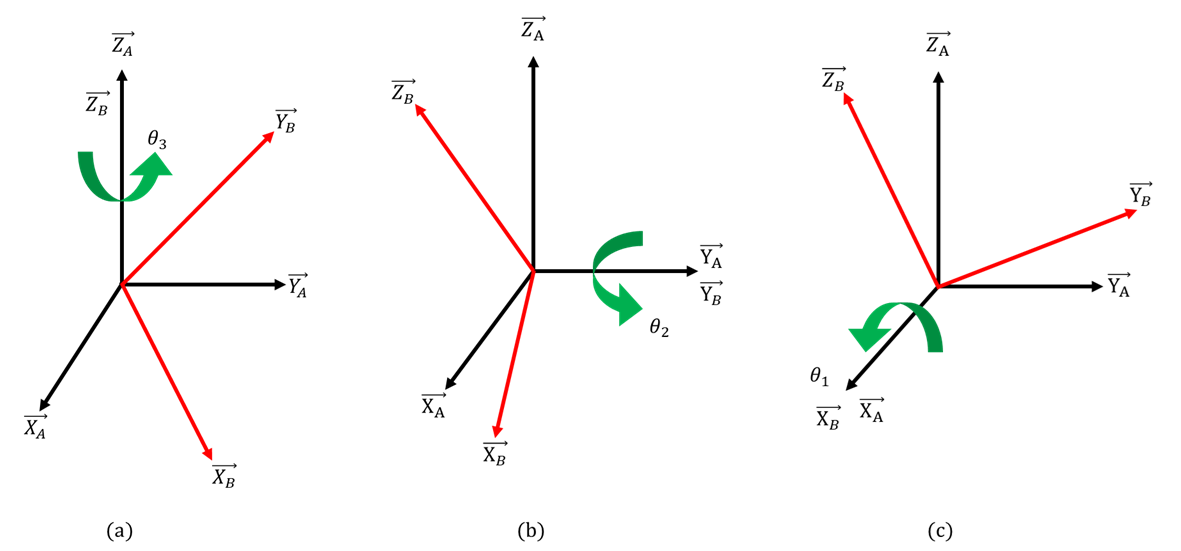
\includegraphics[width=0.90\linewidth]{2 Formulacao do problema/Imagens/Rotacao_XYZ.png}
% \caption
% {Rotação extrínseca XYZ: (a) rotação em Z; (b) rotação em Y; (c) rotação em X no referencial inercial. Adaptado de \cite{craig2005}.}
%     \label{fig:Rotacao_XYZ}
% \end{figure}

\subsubsection{Composição de rotações em sequência}
\label{sec:composicao_rotacoes_sequencia}
No manipulador robótico, cada elo possui um sistema de coordenadas local. Para obter a posição e a orientação do efetuador final (\emph{end-effector}) em relação à base, é necessário compor as rotações sucessivas, como exemplificado:

\eqn{eq:exemplo_composicao}
{{}^0 \mathbf{R}_n =
{}^0 \mathbf{R}_1
{}^1 \mathbf{R}_2  \, ... \,
{}^{n-1} \mathbf{R}_n.}

Para exemplificação, será utilizada a sequência de rotações extrínsecas \emph{ZYX}, também conhecida como \emph{yaw, pitch e roll}, com três ângulos definidos ($\psi,\theta,\phi$), podendo ser descrita como:
\begin{equation}
{}^A \mathbf{R}_{B(\text{zyx})}(\psi,\theta,\phi) = \mathbf{R}_z(\psi)\,\mathbf{R}_y(\theta)\,\mathbf{R}_x(\phi).
\label{eq:rotacao_ZYX1}
\end{equation}

Neste trabalho, adota-se a convenção extrínseca, ou seja, a ordem de aplicação das rotações é da direita para a esquerda — começando pela matriz mais à direita. Assim, a rotação em torno de $Z$ (yaw) é aplicada primeiro, seguida pela rotação em torno de $Y$ (pitch), e por fim pela rotação em torno de $X$ (roll).

Substituindo\fn{Para simplificação de notação: $\cos(\alpha)=c(\alpha)$, $\sin(\alpha)=s(\alpha)$.}
as matrizes elementares, obtém-se:
\begin{equation}
    \label{rotacao_ZYX2}
{}^A \mathbf{R}_{B(\text{zyx})}(\psi,\theta,\phi) =
\begin{bmatrix}
c\psi & -s\psi & 0 \\
s\psi &  c\psi & 0 \\
0     &  0     & 1
\end{bmatrix}
\begin{bmatrix}
 c\theta & 0 & s\theta \\
 0       & 1 & 0       \\
-s\theta & 0 & c\theta
\end{bmatrix}
\begin{bmatrix}
1 & 0      & 0       \\
0 & c\phi & -s\phi  \\
0 & s\phi &  c\phi
\end{bmatrix}.
\end{equation}

Resultando em:
\begin{equation}
    \label{rotacao_ZYX3}
{}^A \mathbf{R}_{B(\text{zyx})}(\psi,\theta,\phi) =
\begin{bmatrix}
c\psi c\theta & c\psi s\theta s\phi - s\psi c\phi & c\psi s\theta c\phi + s\psi s\phi \\
s\psi c\theta & s\psi s\theta s\phi + c\psi c\phi & s\psi s\theta c\phi - c\psi s\phi \\
-\,s\theta    & c\theta s\phi                      & c\theta c\phi
\end{bmatrix}.
\end{equation}

\begin{figure}[ht]
\centering
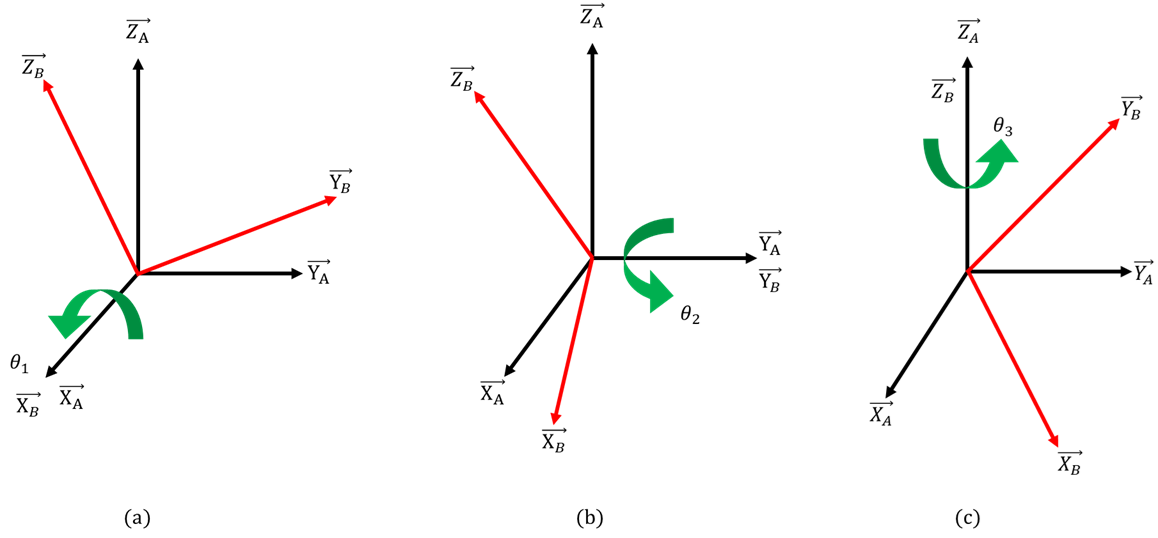
\includegraphics[width=0.70\linewidth]{2 Formulacao do problema/Imagens/Rotacao_ZYX.png}
\caption
{Rotação extrínseca ZYX: (a) rotação em Z (yaw); (b) rotação em Y (pitch); (c) rotação em X (roll) no sistema inercial. Adaptado de \cite{craig2005}.}
    \label{fig:Rotacao_ZYX}
\end{figure}

A figura \eqref{fig:Rotacao_ZYX} mostra o sistema inercial (preto) em relação ao sistema rotacionado (vermelho) para a sequência ZYX. Dessa forma, quando uma origem de um sistema é transladado entre as origens dos referenciais, é necessário ter o vetor posição de uma origem em relação à outra.
\begin{figure}[ht]
    \centering
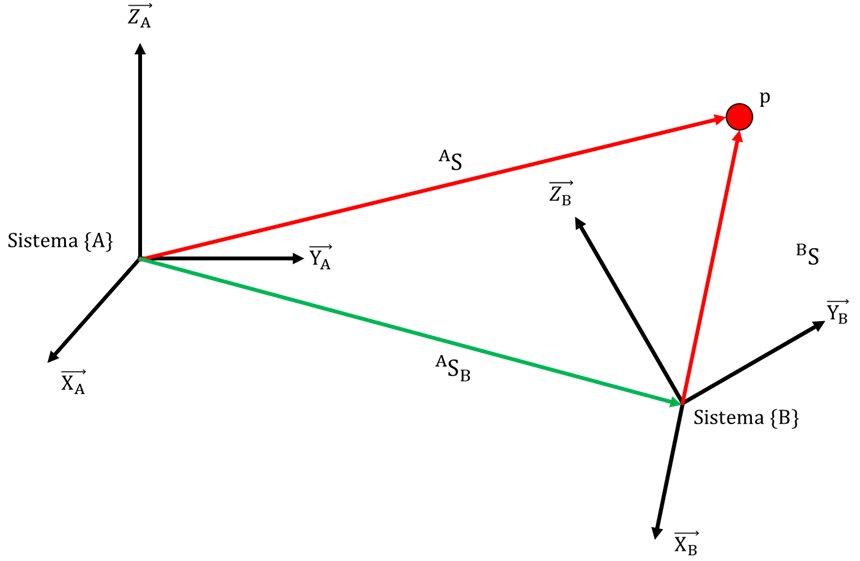
\includegraphics[width=0.50\linewidth]{2 Formulacao do problema/Imagens/DeslocamentoAparaB.png}
    \caption{Representação de um vetor posição em relação a dois sistemas.}
    \label{fig:Deslocamento_AparaB}
\end{figure}

Para encontrar a posição do Sistema $\{A\}$:
\begin{equation}
{}^A \vec{S} = {}^A \mathbf{R}_B \, {}^B \vec{S} + {}^A \vec{S}_B
\end{equation}

Onde ${}^A \vec{p}_B$ é a translação do frame $\{B\}$ em relação a $\{A\}$; ${}^B \vec{p}$ é a coordenada do ponto expressa em $\{B\}$; e ${}^A \vec{p}$ é a coordenada do mesmo ponto expressa em $\{A\}$.


%==================================================
%----- Derivadas parciais de R na sequencia ZYX
%==================================================
\subsubsection{Derivadas parciais de \(\mathbf R\) na sequência ZYX}

Seja
\begin{equation}
\mathbf R(\psi,\theta,\phi)=\mathbf R_z(\psi)\,\mathbf R_y(\theta)\,\mathbf R_x(\phi),
\end{equation}
com as matrizes elementares de rotação
% $\mathbf R_x,\mathbf R_y,\mathbf R_z$ apresentadas em
\eqref{eq:rotacao_X}, \eqref{eq:rotacao_Y} e \eqref{eq:rotacao_Z}, as derivadas parciais são expressas, respectivamente, matematicamente por:

\begin{equation}
    \label{eq:derivada_rz}
\frac{\partial \mathbf R}{\partial \psi}=\mathbf R'_z(\psi)\,\mathbf R_y(\theta)\,\mathbf R_x(\phi),
\end{equation}

\begin{equation}
    \label{eq:derivada_ry}
\frac{\partial \mathbf R}{\partial \theta}=\mathbf R_z(\psi)\,\mathbf R'_y(\theta)\,\mathbf R_x(\phi),
\end{equation}

\begin{equation}
\label{eq:derivada_rx}
\frac{\partial \mathbf R}{\partial \phi}=\mathbf R_z(\psi)\,\mathbf R_y(\theta)\,\mathbf R'_x(\phi),
\end{equation}

onde cada termo pode ser formulado como:
\begin{equation}
    \label{eq:matriz_derivada_rz}
\mathbf R'_z(\psi)=
\begin{bmatrix}
-\sin\psi & -\cos\psi & 0\\
 \cos\psi & -\sin\psi & 0\\
 0&0&0
\end{bmatrix},
\end{equation}

\begin{equation}
    \label{eq:matriz_derivada_ry}
\mathbf R'_y(\theta)=
\begin{bmatrix}
-\sin\theta&0&\cos\theta\\
0&0&0\\
-\cos\theta&0&-\sin\theta
\end{bmatrix},
\end{equation}

\begin{equation}
    \label{eq:matriz_derivada_rx}
\mathbf R'_x(\phi)=
\begin{bmatrix}
0&0&0\\
0&-\sin\phi&-\cos\phi\\
0&\cos\phi&-\sin\phi
\end{bmatrix},
\end{equation}


%==================================================
%----- Derivada temporal
%==================================================
\subsubsection{Derivada temporal e mapeamentos de velocidades angulares}
A derivada temporal é realizada nas derivadas parciais apresentadas em \eqref{eq:derivada_rz}, \eqref{eq:derivada_ry} e \eqref{eq:derivada_rx}:
\begin{equation}
\dot{\mathbf R}=\frac{\partial \mathbf R}{\partial \psi}\dot\psi+\frac{\partial \mathbf R}{\partial \theta}\dot\theta+\frac{\partial \mathbf R}{\partial \phi}\dot\phi.
\end{equation}
Como $\mathbf R^\top\mathbf R=\mathbf I$, vale a identidade clássica:

\begin{equation}
\dot{\mathbf R}=\mathbf R\,[\vec\omega]_\times,
\end{equation}

sendo:
\begin{equation}
[\vec\omega]_\times=
\begin{bmatrix}
0&-\omega_z&\ \omega_y\\
\ \omega_z&0&-\omega_x\\
-\omega_y&\ \omega_x&0
\end{bmatrix}.
\end{equation}

Para a sequência ZYX, os mapeamentos entre $[\dot\phi,\dot\theta,\dot\psi]^\top$ é dado por:
\begin{equation}
\begin{bmatrix}\omega_x\\ \omega_y\\ \omega_z\end{bmatrix}=
\underbrace{\begin{bmatrix}
1 & 0 & -\sin\theta\\
0 & \cos\phi & \sin\phi\,\cos\theta\\
0 & -\sin\phi & \cos\phi\,\cos\theta
\end{bmatrix}}_{\displaystyle \mathbf T_{zyx}(\phi,\theta)}
\begin{bmatrix}\dot\phi\\ \dot\theta\\ \dot\psi\end{bmatrix},
\end{equation}

enquanto que para a velocidade angular da base ($frame \{0\}$) o modelo pode ser descrito como: 
\begin{equation}
\begin{bmatrix}\dot\phi\\ \dot\theta\\ \dot\psi\end{bmatrix}=
\underbrace{\begin{bmatrix}
1 & \sin\phi\tan\theta & \cos\phi\tan\theta\\
0 & \cos\phi & -\sin\phi\\
0 & \sin\phi/\cos\theta & \cos\phi/\cos\theta
\end{bmatrix}}_{\displaystyle \mathbf W_{zyx}(\phi,\theta)}
\begin{bmatrix}\omega_x\\ \omega_y\\ \omega_z\end{bmatrix}.
\end{equation}

\subsubsection{Singularidade}
Em ZYX ocorre singularidade cinemática para
$\theta=\pm\frac{\pi}{2}$ e ($cos\theta=0$),
quando $\mathbf W_{zyx}$ não pode ser invertido.
Essa limitação motiva o uso de quaternions na malha de controle de atitude.






%==================================================
%----- Matriz de transformação homogênea
%==================================================
\section{Matriz de transformação homogênea}
A matriz de transformação homogênea é utilizada como uma forma geral de construção para realizar a rotação e a translação ao mesmo tempo,
e é definida como:
\begin{equation}
\label{eq:def_T_AB}
{}^{A}\mathbf{T}_{B} =
\begin{bmatrix}
{}^{A}\mathbf{R}_{B} & {}^{A}\vec{p}_{B} \\
\vec{0}^{\,T} & 1
\end{bmatrix}.
\end{equation}

Ela é útil para encontrar o ponto $\{p\}$ em relação ao Sistema $\{A\}$, define-se:
\begin{equation}
\begin{bmatrix}
{}^A \vec{p} \\[2pt] 1
\end{bmatrix}
=
{}^A \mathbf{T}_B
\begin{bmatrix}
{}^B \vec{p} \\[2pt] 1
\end{bmatrix}.
\end{equation}

A composição da matriz homogênea segue o mapeamento dos \emph{frames}:
\begin{equation}
\label{eq:comp_T}
{}^{A}\mathbf{T}_{C} = {}^{A}\mathbf{T}_{B}\,{}^{B}\mathbf{T}_{C}.
\end{equation}

Levando em consideração que agora é possível estabelecer um ponto no espaço através da matriz de transformação homogênea, de forma similar, a pose do Efetuador $\{E\}$ em relação à base $\{B\}$, se dá conforme a notação DH, é o produto de todas as matrizes $A_i$, como pode ser definido:
\begin{equation}
    \label{eq:produtorio_generico}
{}^{0}\mathbf{T}_E(q)= \prod_{i=1}^{n} \mathbf{A}_i(q)
= \mathbf{A}_1(q)\,\mathbf{A}_2(q)\,\cdots\,\mathbf{A}_n(q).
\end{equation}

\begin{equation}
\label{eq:extract_R_p}
\mathbf{R}_{E}(q)=\big[{}^{0}\mathbf{T}_{E}(q)\big]_{1:3,\,1:3},
\qquad
\vec{p}_{E}(q)=\big[{}^{0}\mathbf{T}_{E}(q)\big]_{1:3,\,4}.
\end{equation}


%==================================================
%----- Derivadas e adjunta em SE(3)
%==================================================
% \subsection{Derivadas e adjunta em SE(3)}
% Para
% \begin{equation}
% \mathbf T=
% \begin{bmatrix}
% \mathbf R   & \vec p\\
% \vec 0^\top & 1
% \end{bmatrix}
% \in SE(3),
% \end{equation}

% é possível definir a torção espacial:
% \begin{equation}
%     \label{eq:torcao_espacial}
% \vec{\mathcal V}_S
% \begin{bmatrix}
%     \vec v_s\\
%     \vec \omega_s
% \end{bmatrix}, 
% \end{equation}

% e a torção corporal:
% \begin{equation}
%     \label{eq:torcao_corporal}
% \vec{\mathcal V}_B=
% \begin{bmatrix}
%     \vec v_B\\
%     \vec \omega_B
% \end{bmatrix},
% \end{equation}

% com operadores $\widehat{\cdot}$ sendo definidos como:
% \begin{equation}
% \widehat{\vec{\mathcal V}}=
% \begin{bmatrix}
%     [\vec\omega]_\times & \vec v \\
%     \vec 0^\top         & 0
% \end{bmatrix}.
% \end{equation}

% Portanto, podem ser utilizadas suas formas compactas:
% \begin{equation}
% \dot{\mathbf T}=\,\widehat{\vec{\mathcal V}}_S\,\mathbf T
% \ =\
% \mathbf T\,\widehat{\vec{\mathcal V}}_B,
% \end{equation}

% sendo:
% \begin{equation}
% \vec{\mathcal V}_S=\mathrm{Ad}_{\mathbf T}\,\vec{\mathcal V}_B,
% \end{equation}

% e a matriz adjunta escrita como:
% \begin{equation}
% \operatorname{Ad}_{T}=
% \begin{bmatrix}
% \mathbf R & [\vec p]_\times \mathbf R\\
% \mathbf 0 & \mathbf R
% \end{bmatrix},
% \qquad
% T=\begin{bmatrix}\mathbf R&\vec p\\ \mathbf 0^\top & 1\end{bmatrix}\in SE(3).
% \end{equation}

% Na cinemática direta
% $^{0}\mathbf T_{E}=\prod_{i=1}^{n}\mathbf A_i(q_i)$,
% obtém-se:
% \begin{equation}
% \dot{\,^{0}\mathbf T_{E}}=
% \sum_{i=1}^n
% \left(\prod_{k=1}^{i-1}\mathbf A_k\right)
% \dot{\mathbf A}_i
% \left(\prod_{k=i+1}^{n}\mathbf A_k\right),
% \end{equation}

% com
% $\dot{\mathbf A}_i=\mathbf A_i\,\widehat{\vec{\mathcal V}}_{B,i}$
% para juntas revolutas
% ($\vec{\mathcal V}_{B,i}=[\,\hat{\vec z}_{i-1},\,\vec 0\,]^\top$)
% e prismáticas
% ($\vec{\mathcal V}_{B,i}=[\,\vec 0,\,\hat{\vec z}_{i-1}\,]^\top$).


%==================================================
%----- Matriz de transformação homogênea DH
%==================================================
\subsection{Matriz de transformação homogênea DH}

A matriz de transformação homogênea $A_i$ possui dimensão de ordem 4 e reúne a rotação em torno de $z_{i-1}$;
a translação ao longo de $z_{i-1}$;
a translação ao longo de $X_{i}$;
e a rotação em torno de $x_{i}$.
O resultado é a matriz $A_i$, que relaciona o \emph{frame} do elo $i$ com o frame do elo anterior ($i-1$).
Portanto, essa matriz possui toda a informação geométrica que define como o elo $i$ está posicionado e orientado em relação ao elo anterior.

Cada elo do manipulador robótico é descrito, de acordo com a convenção de Denavit-Hartenberg clássica, através de uma matriz de transformação homogênea, $A_i$ e sua forma expandida é definida como:
\begin{equation}
    \label{eq:matrizTransformacaoHomogenea}
\mathbf{A}_i =
\begin{bmatrix}
\cos\theta_i & -\sin\theta_i \cos\alpha_i &
\sin\theta_i \sin\alpha_i & a_i \cos\theta_i \\
\sin\theta_i & \cos\theta_i \cos\alpha_i  &
-\cos\theta_i \sin\alpha_i & a_i \sin\theta_i \\
0 & \sin\alpha_i & \cos\alpha_i & d_i \\
0 & 0 & 0 & 1
\end{bmatrix}.
\end{equation}

E a forma reduzida da matriz \eqref{eq:matrizTransformacaoHomogenea} pode ser reescrita conforme:
\begin{equation}
\label{eq:matrizTransformacaoHomogenea_reduzida}
\mathbf{A}_i = 
\begin{bmatrix}
\mathbf{R} & \vec{p} \\
\vec{0}^{\,T} & 1
\end{bmatrix},
\end{equation}

onde:
\begin{itemize}
    \item $\mathbf{R}_{(3\times 3)}$: submatriz de rotação que descreve o frame $i$ relativo ao frame $i-1$.
    \item $\mathbf{p}_{(3\times 1)}$: vetor posição que descreve  o frame $i$ relativo ao frame $i-1$.
\end{itemize}

Portanto, o equacionamento para obter a pose do efetuador em relação à base é definido como:

\begin{equation}
{}^{0}\!T_i(q)=
{}^{0}\!T_{i-1}(q)
A_i(q).
\end{equation}

Sendo que:
\begin{equation}
{}^{0}\!T_0 = I_{4}.
\end{equation}

A formulação apresentada será aplicada na seção a seguir para relacionar diferentes sistemas de referência orbitais - como o Inercial e o LVLH - fundamentais para operações de RVD/B.
